\newpage
\section{Securing Certificates}


\begin{Def}[Euler's Totient Function]

    \label{def:euler}
    The \textbf{Euler's Totient Function} $\phi(n)$ is the number of positive integers less than $n$ that are coprime to $n$.
    For a prime number $p$, $\phi(p)=p-1$.
    For two distinct prime numbers $p$ and $q$, $\phi(p \cdot q)=(p-1)(q-1)$.
    For a prime power $p^k$, $\phi(p^k)=p^{k-1}(p-1)$.
\end{Def}

\begin{theo}[Modular Multiplicative Inverse]

    \label{def:mod_inv}
    The \textbf{Modular Multiplicative Inverse} of an integer ($a$ modulo $m$) is an integer $x$, s.t., $a \cdot x \equiv 1 (\text{mod } m)$.
    Inverse exists if and only if $\gcd(a,m)=1$ (coprime).\\

    \noindent
    \textbf{Denoted:} $a^{-1}\iff a \cdot a^{-1} \equiv 1 (\text{mod } m)$.
\end{theo}

\begin{Def}[Rivest-Shamir-Adleman (RSA)]

    \label{def:rsa}
    The \textbf{RSA} algorithm is a public-key cryptosystem. First described in 1977 by Ron \textbf{R}ivest, Adi \textbf{S}hamir, and Leonard \textbf{A}dleman at MIT.
    The RSA algorithm involves three steps: key generation, encryption, and decryption. It goes as follows:
    \begin{enumerate}
        \item \textbf{Key Generation:} 
        \begin{enumerate}
            \item Select two large prime numbers $p$ and $q$.
            \item Compute $n=p \cdot q$.
            \item Compute $\phi(n)=(p-1)(q-1)$.
            \item Select an integer $e$ such that $1<e<\phi(n)$ and $\gcd(e,\phi(n))=1$.
            \item Compute $d$ as $d \equiv e^{-1} \text{ mod } \phi(n)$.
            \item The public key is $(n,e)$ and the private key is $(n,d)$.
        \end{enumerate}
        \item \textbf{Encryption:} 
        \begin{enumerate}
            \item To encrypt a message $m$, compute $c \equiv m^e (\text{ mod } n)$.
        \end{enumerate}
        \item \textbf{Decryption:} 
        \begin{enumerate}
            \item To decrypt a ciphertext $c$, compute $m \equiv c^d (\text{ mod } n)$.
        \end{enumerate}
    \end{enumerate}
    \noindent
    For emphasis:
    $$(m^e)^d \equiv m^{ed} \equiv m^1 (\text{ mod } n)$$,
    \noindent
    The security of RSA relies on the practical difficulty of factoring the product of two large prime numbers, the factoring problem. \hfill \cite{RSA}
\end{Def}

\newpage 

\begin{Example}[RSA Encryption and Decryption]
    \label{ex:rsa_example}
    The following is an example of the RSA algorithm, including key generation, encryption, and decryption.
    Smaller primes are chosen for brevity:
    \begin{enumerate}
        \item \textbf{Key Generation:}
        \begin{enumerate}
            \item Choose two distinct prime numbers: $p = 61$ and $q = 53$.
            \item Compute $n = p \cdot q$:
            \[
            n = 61 \cdot 53 = 3233.
            \]
            \item Compute the totient function $\phi(n)$ as:
            \[
            \phi(n) = (p-1)(q-1) = 60 \cdot 52 = 780.
            \]
            \item Choose an integer $e$ such that $1 < e < \phi(n)$ and $\gcd(e, \phi(n)) = 1$:
            \[
            e = 17.
            \]
            \item Compute $d$, the modular multiplicative inverse of $e \text{ mod } \phi(n)$:
            \[
            d \equiv e^{-1} \text{mod } \phi(n) \implies d = 413.
            \]
            \item The public key is $(n, e) = (3233, 17)$, and the private key is $(n, d) = (3233, 413)$.
        \end{enumerate}
        
        \item \textbf{Encryption:}
        \begin{enumerate}
            \item To encrypt a plaintext message $m$, compute:
            \[
            c \equiv m^e (\text{mod } n).
            \]
            For $m = 65$, we calculate:
            \[
            c = 65^{17} \text{mod } 3233 = 2790.
            \]
        \end{enumerate}

        \item \textbf{Decryption:}
        \begin{enumerate}
            \item To decrypt a ciphertext $c$, compute:
            \[
            m \equiv c^d (\text{mod } n).
            \]
            For $c = 2790$, we calculate:
            \[
            m = 2790^{413} \text{mod} 3233 = 65.
            \]
        \end{enumerate}
    \end{enumerate}
    \noindent
    This example demonstrates the RSA encryption and decryption process,
    where a message $m = 65$ is encrypted and successfully decrypted back to its original value. \hfill{}
\end{Example}


\newpage

\begin{theo}[RSA Security Definition]

    \underline{RSA provides authenticity} of a data source; However,
    \begin{center}
        \textbf{RSA does not provide confidentiality or integrity.}
    \end{center}
    \noindent
\end{theo}

\noindent
In this case certificates are meant to be public so confidentiality is not a concern;
However, integrity is. For integrity, \textbf{HMACs} are used. The hashing algorithm 
used on certificates is often \textbf{SHA-256}.

\begin{Def}[Secure Hash Algorithm 256 (SHA-256)]

    \label{def:sha256}
    The \textbf{SHA-256} algorithm is a cryptographic hash function belonging to the SHA-2 (Secure Hash Algorithm 2) family, standardized by NIST in 2001.  
    It produces a fixed-length 256-bit hash value from an input message of any size. The algorithm is as follows:
    \begin{enumerate}
        \item \textbf{Initialization:}
        \begin{enumerate}
            \item Define the \textbf{message input} as a bit string of arbitrary length.
            \item Pad the message so that its length (in bits) is congruent to $448$ mod $512$.
            \item Append the 64-bit representation of the original message length to create a message of size divisible by 512 bits.
        \end{enumerate}
        
        \item \textbf{Message Schedule:}
        \begin{enumerate}
            \item Divide the padded message into blocks of 512 bits each.
            \item Each block is processed in 64 rounds using a schedule of 32-bit words $W_0, \dots, W_{63}$, which are derived from the 512-bit block.
        \end{enumerate}

        \item \textbf{Hash Computation:}
        \begin{enumerate}
            \item Initialize eight 32-bit \textbf{hash values} $H_0, H_1, \dots, H_7$ to predefined constants.
            \item For each message block:
            \begin{enumerate}
                \item Perform 64 rounds of operations involving:
                \begin{itemize}
                    \item Bitwise logical functions (\texttt{AND}, \texttt{OR}, \texttt{XOR}),
                    \item Modular addition,
                    \item Circular shifts and rotations.
                \end{itemize}
            \end{enumerate}
        \end{enumerate}
        
        \item \textbf{Output:}
        \begin{enumerate}
            \item After processing all blocks, concatenate the final hash values:
            \[
            \text{SHA-256}(M) = H_0 \| H_1 \| H_2 \| H_3 \| H_4 \| H_5 \| H_6 \| H_7.
            \]
            \item The output is a 256-bit (32-byte) fixed-length hash digest.
        \end{enumerate}
    \end{enumerate}
\end{Def}

\newpage

\begin{theo}[Digital Signatures with RSA and SHA-256]

    \label{def:rsa_sha256}
    Digital signatures are used to verify the authenticity and integrity of a message. Using RSA and SHA-256, the process is as follows:
    \begin{enumerate}
        \item \textbf{Hashing:}
        \begin{enumerate}
            \item The sender computes the SHA-256 hash of the message or certificate:
            \[
            H = \text{SHA-256}(\text{Message}).
            \]
        \end{enumerate}
        
        \item \textbf{Signing:}
        \begin{enumerate}
            \item The sender encrypts the hash $H$ using their RSA private key to generate the digital signature:
            \[
            S = H^d \mod n.
            \]
        \end{enumerate}
        
        \item \textbf{Transmission:}
        \begin{enumerate}
            \item The sender sends the message and the digital signature $(\text{Message}, S)$.
        \end{enumerate}
        
        \item \textbf{Verification:}
        \begin{enumerate}
            \item The recipient computes the SHA-256 hash of the received message:
            \[
            H' = \text{SHA-256}(\text{Message}).
            \]
            \item The recipient decrypts the digital signature $S$ using the sender's RSA public key:
            \[
            H'' = S^e \mod n.
            \]
            \item The recipient verifies the signature by checking if:
            \[
            H' = H''.
            \]
            If the hashes match, the message is authentic and unaltered.
        \end{enumerate}
    \end{enumerate}
    \noindent
    In Short:
    \begin{itemize}
        \item \textbf{Sender:} Specifies an HMAC and signs the digest with their private key.
        \item \textbf{Receiver:} Computes the HMAC and decrypts the signature to see if the hashes match.
    \end{itemize}
\end{theo}

\newpage 

\begin{Def}[Brief History of Hashing Algorithms]

    \label{def:hashing_history}
    Hashing algorithms are essential cryptographic tools that map data of arbitrary size to fixed-size hash values.
    Over time, vulnerabilities in older algorithms have driven the development of more secure alternatives.

    \textbf{MD5} (Message Digest Algorithm 5), introduced in 1991, quickly became popular for checksums
    and data integrity checks. However, it is considered insecure due to susceptibility to
    \textit{collision attacks}, where two different inputs produce the same hash.

    Similarly, \textbf{SHA-1} (Secure Hash Algorithm 1), released by NIST in 1995, generated 160-bit hash values. By the mid-2000s,
    researchers demonstrated its vulnerability to collisions.

    The \textbf{SHA-2} family, introduced in 2001, offered stronger 256-bit (SHA-256) and 512-bit (SHA-512) outputs.
    Despite its robustness, skepticism arose because SHA-2 was designed by the U.S. National Security Agency (NSA), prompting concerns about potential backdoors.

    To address these concerns, NIST held a public competition, resulting in the standardization of \textbf{SHA-3} in 2015.  \hfill \cite{codesigningstore2024hashcomparison}
\end{Def}



\section{Establishing a Secure Connection HTTPS}

\begin{Def}[TLS Handshake Protocol]

    \label{def:tls_handshake}
    The \textbf{TLS Handshake Protocol} is a key exchange protocol that allows two parties to establish
    a secure connection. First a \textbf{TCP handshake} to establish a connection. Then a 
    ``\textbf{Client Hello}'' message is sent, presenting the following parameters:
    \begin{itemize}
        \item Supported TLS versions, cipher suites.
    \end{itemize}
    The server responds with a ``\textbf{Server Hello}'' message, containing:
    \begin{itemize}
        \item  Choosing TLS versions, and a cipher suite.
    \end{itemize}

    \noindent
    The server also sends its certificate, which the client verifies using the PKI. Then a \textbf{Server Hello Done} message is sent, 
    and waits for the client to respond. The key exchange begins:

    \begin{itemize}
        \item RSA Method:The client generates a \textbf{pre-master secret} and encrypts it with the server's public key. The server decrypts the pre-master secret using its private key.
        The client may also use DHE instead.
        \item Both parties signal a \textbf{Change Cipher Spec} message, indicating the switch to encrypted communication.
    \end{itemize}
    
    The client sends a \textbf{Finished} message, which is encrypted with the negotiated algorithms and keys. The server decrypts the message and sends its own \textbf{Finished} message. If the server's message is
    successfully decrypted, the handshake is complete, and the secure connection is established. \hfill \cite{bytebytego2024ssl_tls_https} \cite{rfc5246}
\end{Def}

\newpage 

\noindent
Here is a visual representation of the TLS 1.2 Handshake Protocol:\\

\vspace{4em}
\hspace{-2em}
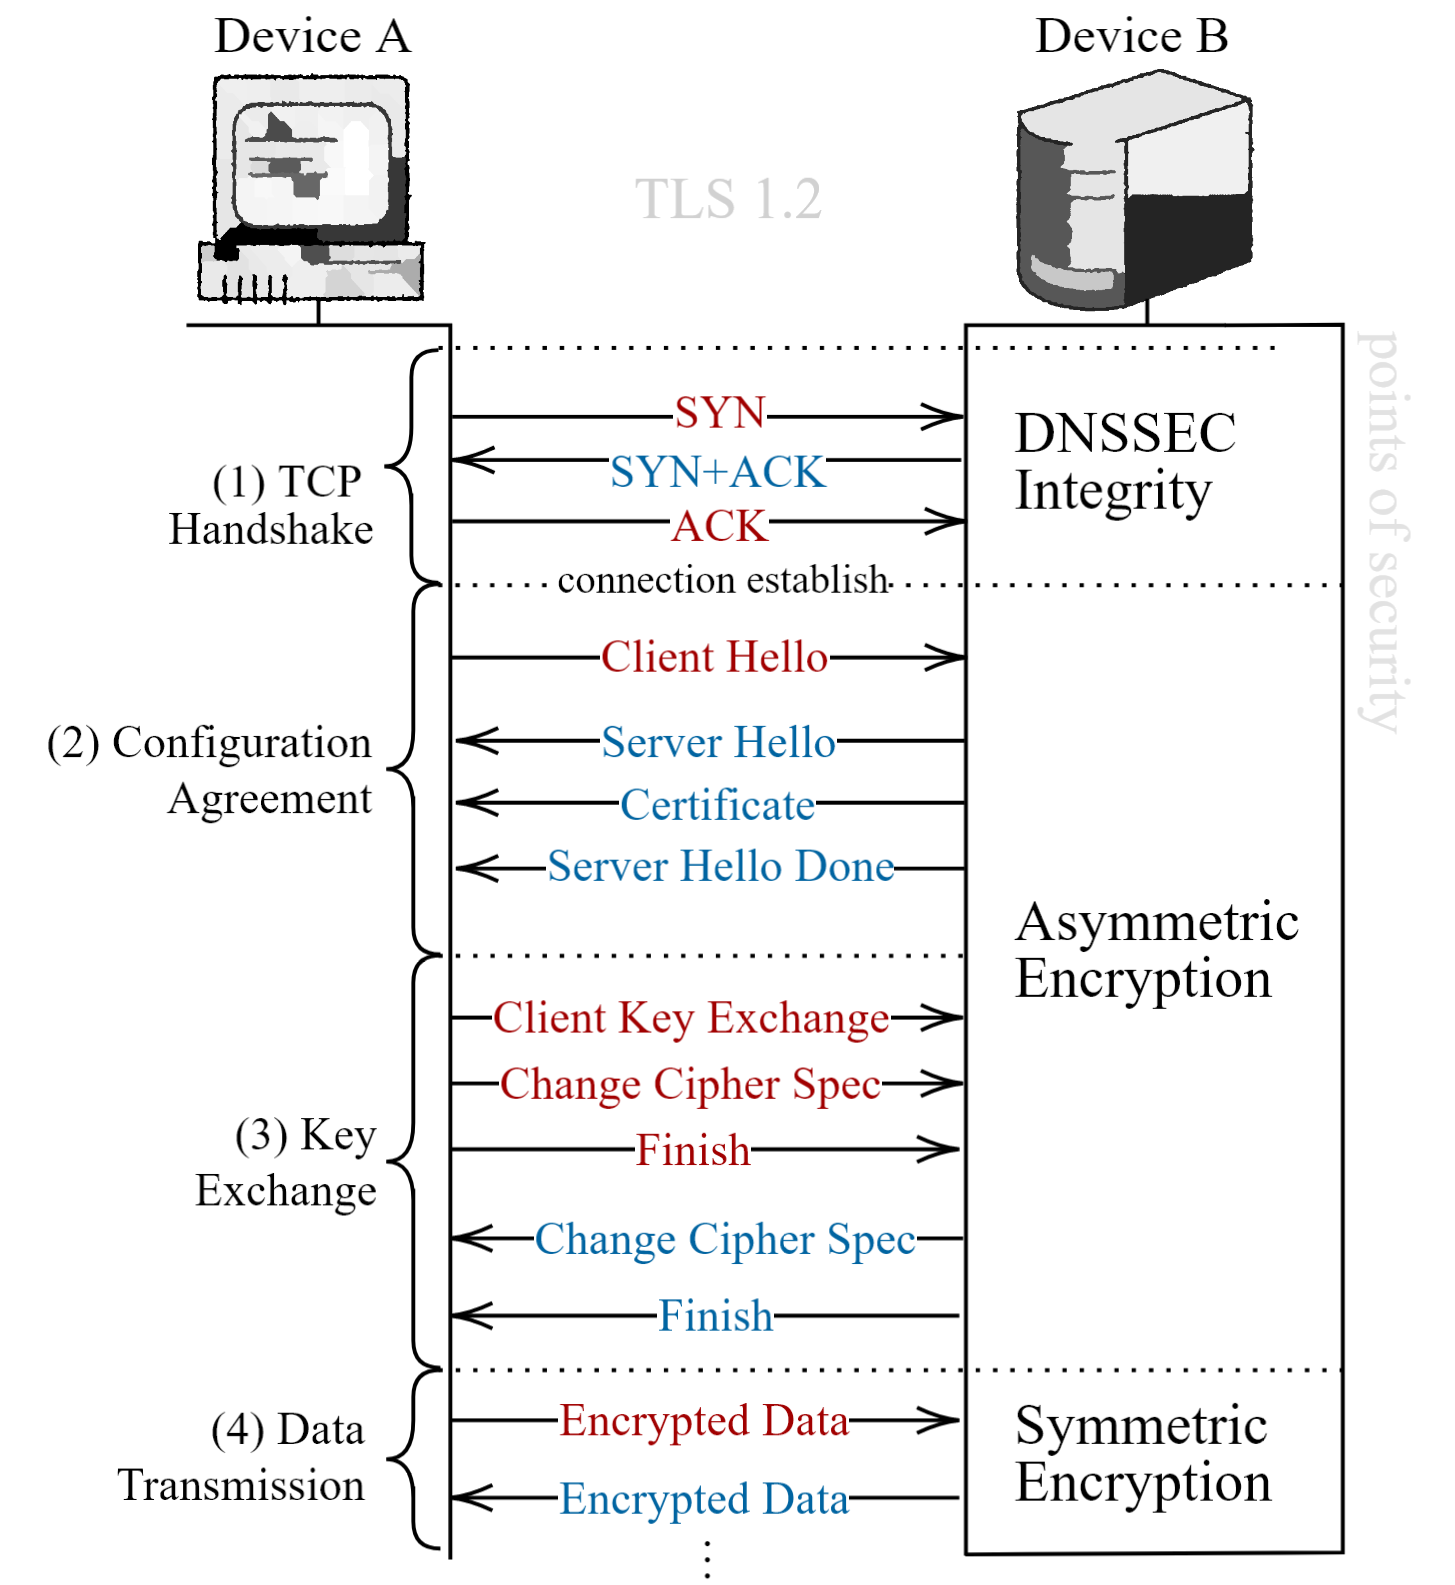
\includegraphics[width=.9\textwidth]{Sections/sec/enc/rsa/tls/tls12.png}

\newpage 

\begin{Def}[Improvements in TLS 1.3 and QUIC]

    \label{def:tls13_quic}
    \begin{enumerate}
        \item \textbf{Improvements in TLS 1.3:}
        \begin{itemize}
            \item \textbf{Reduced Handshake Latency:} 
            \begin{itemize}
                \item The \textbf{Client Key Exchange} and the \textbf{Change Cipher Spec} steps are merged into the initial \textbf{ClientHello} and \textbf{ServerHello} messages.
                \item The client sends the \textbf{key share} (for Diffie-Hellman Ephemeral) in the first message, enabling a \textbf{1-RTT (One Round-Trip Time)} handshake.
            \end{itemize}
            \item \textbf{Zero Round-Trip Time (0-RTT):}
            For resumed connections, clients can send encrypted application data immediately in the first message, reducing the handshake to \textbf{0-RTT}.
            \item \textbf{Forward Secrecy:}
            TLS 1.3 enforces the use of ephemeral Diffie-Hellman (DHE or ECDHE) key exchange, providing \textbf{Perfect Forward Secrecy}.
            \item \textbf{Simplified Cipher Suites:}
            Only modern cipher suites (e.g., AES-GCM, ChaCha20-Poly1305) are supported, enhancing security and reducing complexity.
        \end{itemize}
        
        \item \textbf{QUIC: A Modern Transport Protocol}
        QUIC (Quick UDP Internet Connections) replaces TCP and integrates \textbf{TLS 1.3} into its protocol stack.
        \begin{itemize}
            \item QUIC combines the transport-layer connection setup and the \textbf{TLS 1.3 handshake} into a single step:
            \begin{itemize}
                \item The \textbf{ClientHello} (including key share) is sent in the first QUIC packet.
                \item The \textbf{ServerHello} (including key share and certificate) is sent in the server's first response.
            \end{itemize}
            \item \textbf{Zero Round-Trip Time (0-RTT):}
            QUIC supports \textbf{0-RTT resumption}.
            \item \textbf{Elimination of TCP Handshake:}
            QUIC operates over \text{UDP}, removing the need for the TCP three-way handshake (SYN → SYN-ACK → ACK).
        \end{itemize}
    \end{enumerate}
    \end{Def}

\vspace{2em}
\textbf{Important things to note thus far:}
\begin{itemize}
    \item \textbf{MACs}: Integrity of data. Requires either a shared secret between two parties or specified hashing algorithm (E.g., SHA-256).
    There is no reversing a hash function, they are one-way functions.
    \item \textbf{Certificates \& Digital Signatures}: Authenticity of data. Requires a public key infrastructure (PKI) to verify the identity of the sender (E.g., RSA).
    \item \textbf{Encryption}: Confidentiality of data. Between parties requires a shared secret key (E.g., AES).
\end{itemize}

    \newpage 

\noindent
The following is a visual representation of the TLS 1.3 and QUIC Handshake Protocols:\\

\vspace{1em}

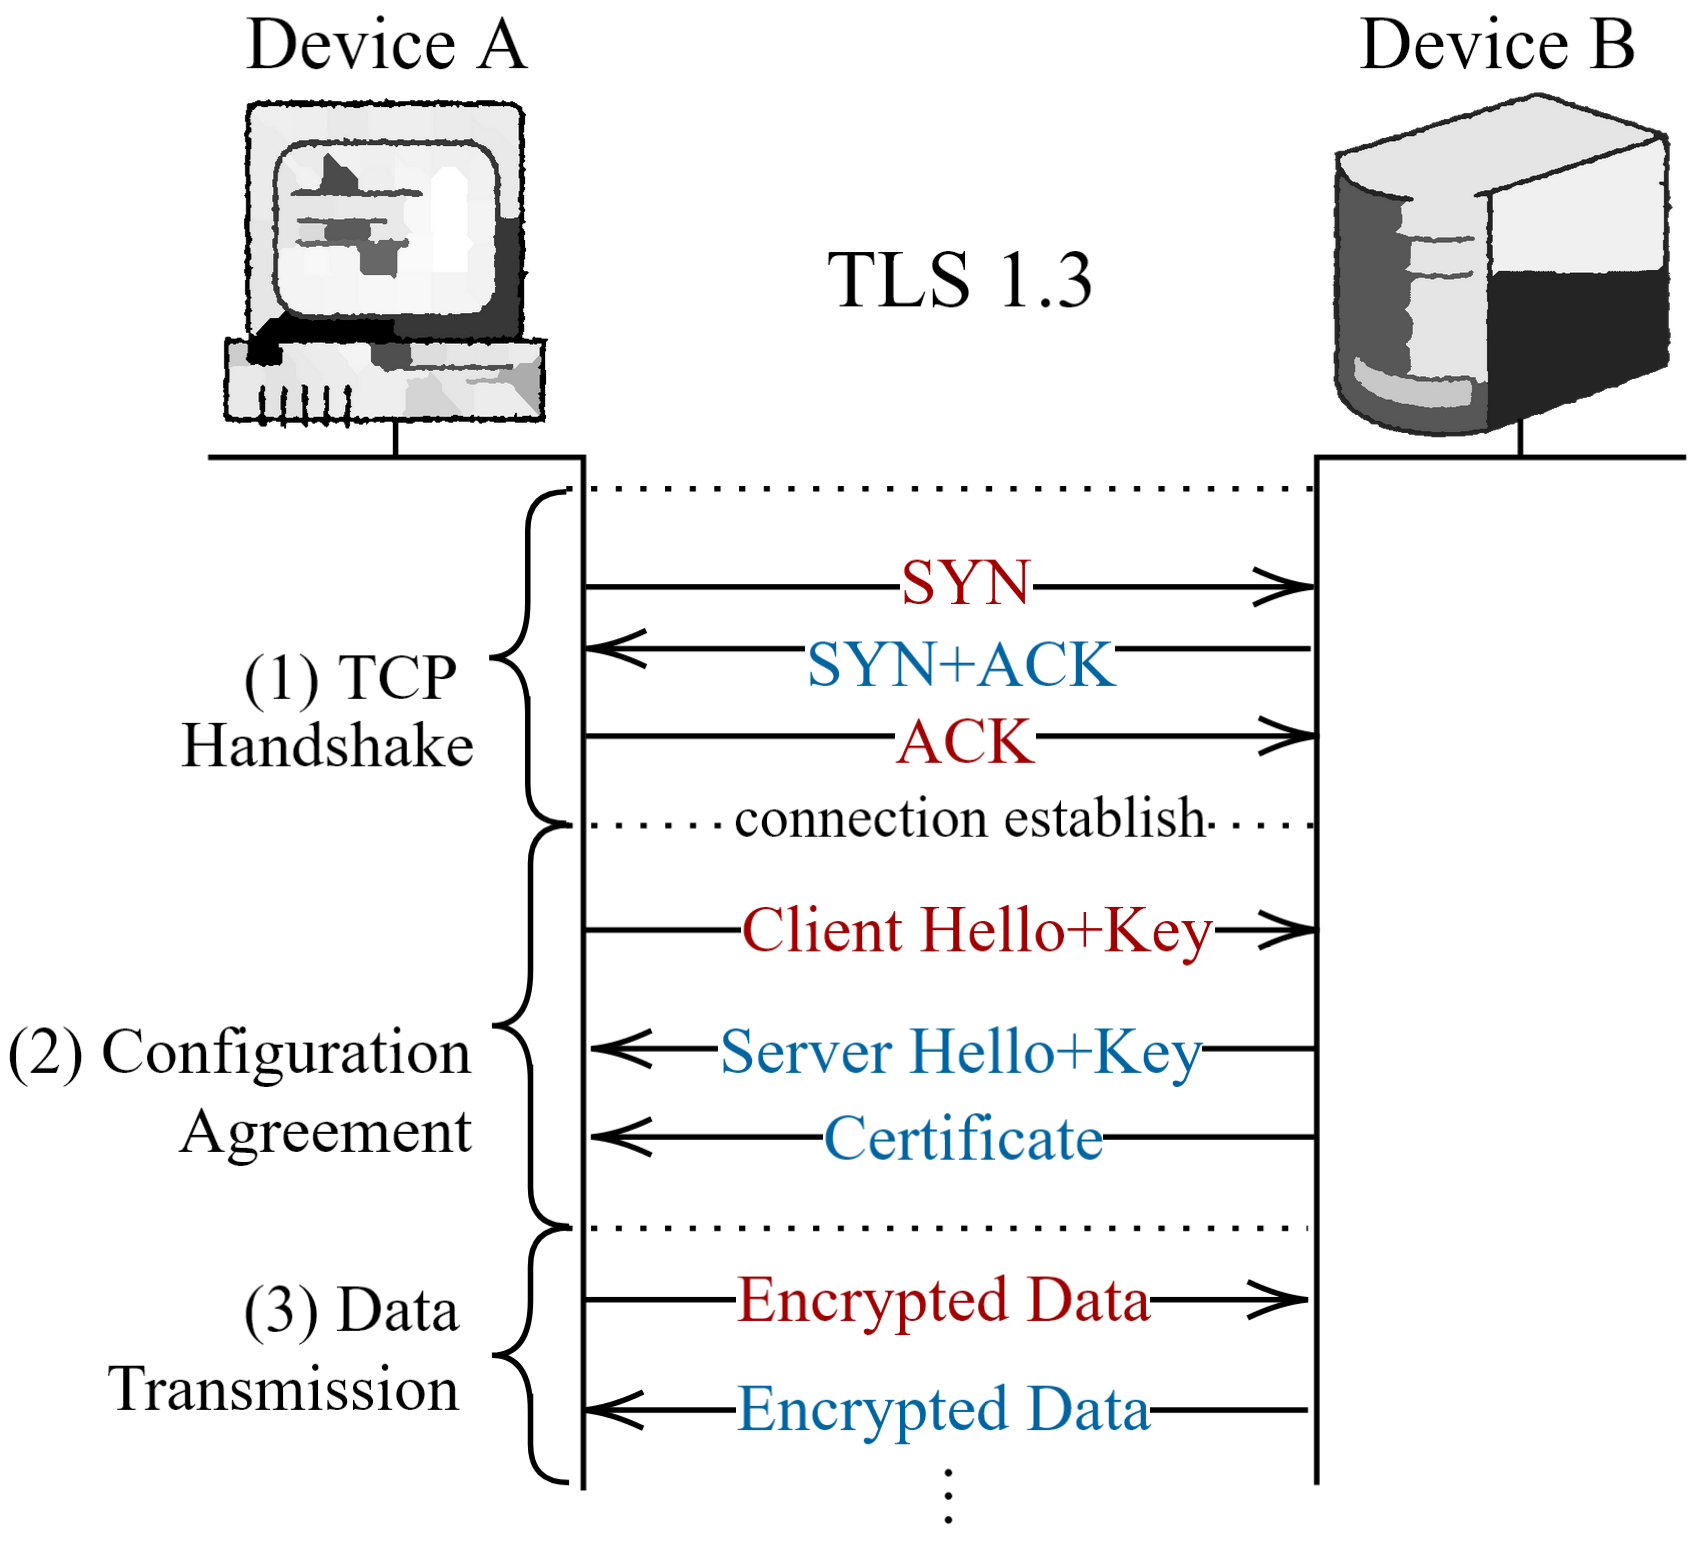
\includegraphics[width=.74\textwidth]{Sections/sec/enc/rsa/tls/tls13.png}

\vspace{1em}
\hspace{1.5em}
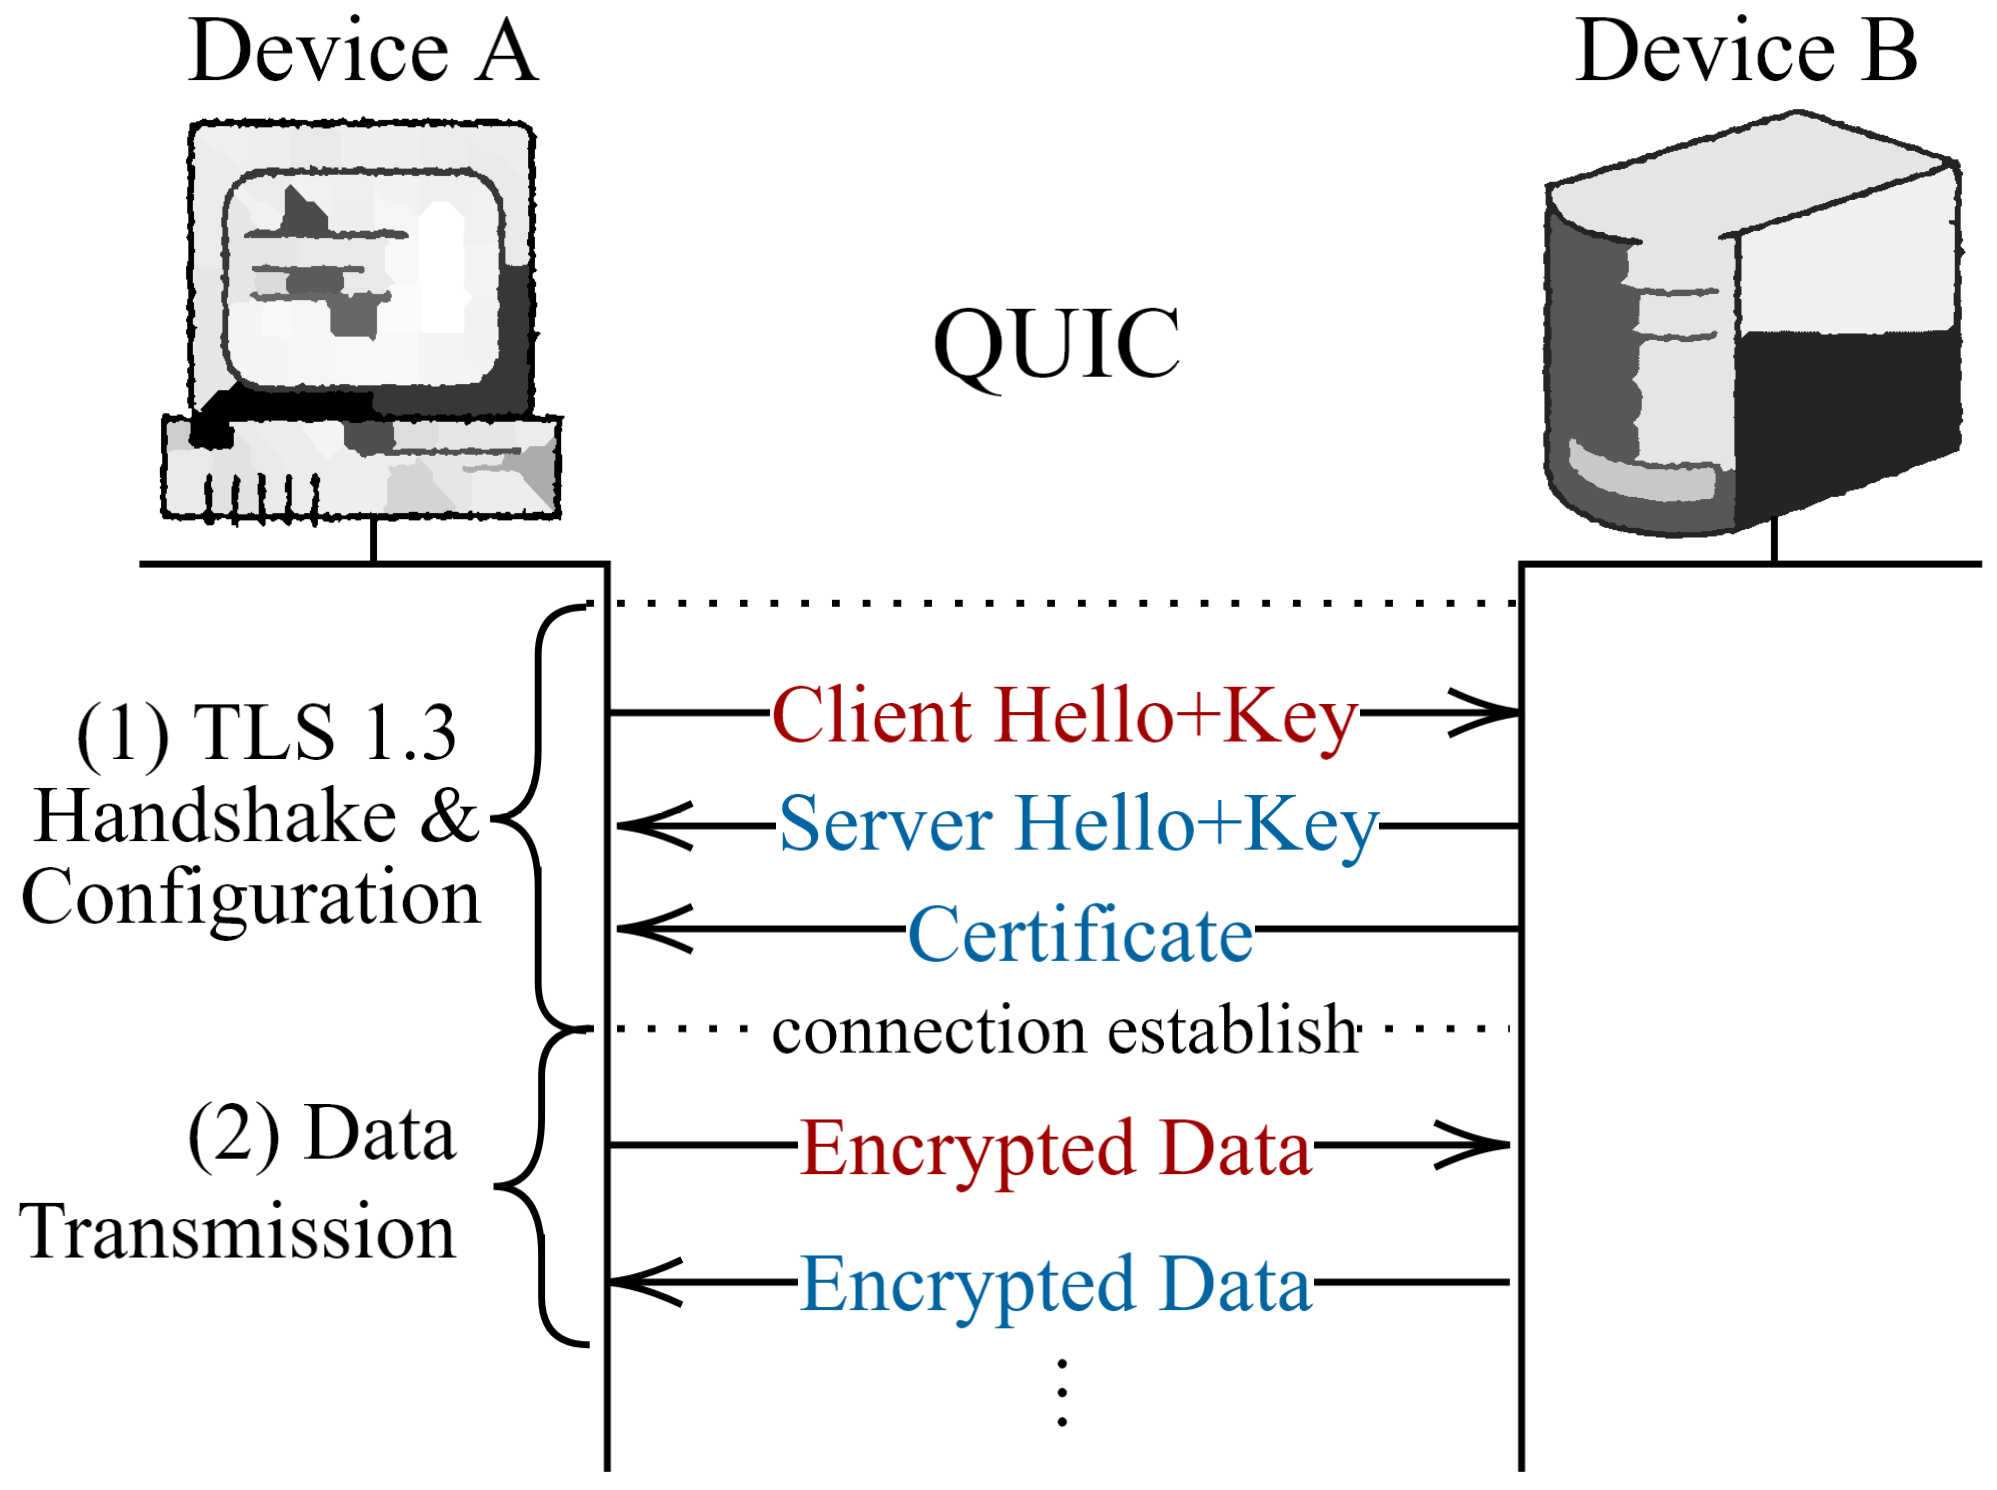
\includegraphics[width=.68\textwidth]{Sections/sec/enc/rsa/tls/quic.png}
    


